\documentclass[12pt]{article}
\usepackage{amsmath, amssymb, graphicx, float, caption, subcaption}
\usepackage{geometry}
\geometry{margin=1in}
\usepackage{booktabs}
\usepackage{verbatim}

\title{ME 340 Heat Transfer Portfolio 2:\\
\large Heating a Black Powder-Coated Hydro Flask Using Sunlight}
\author{Nate Lehnhof\\
ME EN 340 - Section 1}
\date{\today}

\begin{document}

\maketitle

\clearpage
\section*{Picture of Real-World Application}
\begin{figure}[H]
\centering
\rotatebox{270}{\includegraphics[width=0.5\textwidth]{figures/bottle.JPG}}
\caption{A black powder-coated Hydro Flask exposed to sunlight. Heat is transferred from sunlight to water inside and lost through convection.}
\end{figure}

\section*{Description of Heat Transfer Process}
Sunlight heats the outer surface of the black powder-coated Hydro Flask. Heat transfer occurs via:
\begin{itemize}
\item \textbf{Radiation:} Solar energy is absorbed by the surface.
\item \textbf{Convection:} Heat is lost from the surface to ambient air through forced convection.
\end{itemize}

\section*{Engineering Problem Statement}
A black hydro flask is left out in the open on a sunny and windy day. Find the \textbf{steady-state water temperature} $T_w$ in the 500 mL black Hydro Flask exposed to sunlight.

\subsection{Problem Approach}
\begin{figure}[H]
\centering
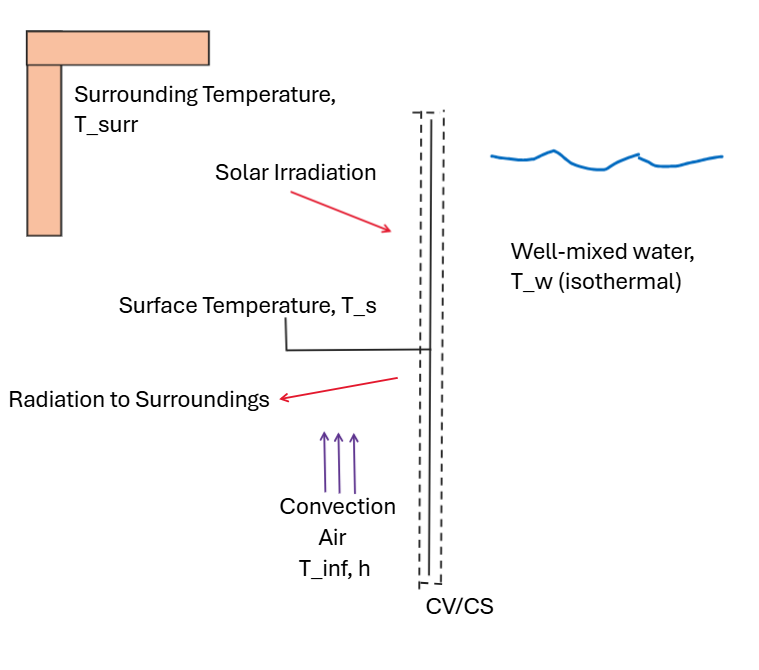
\includegraphics[width=0.7\textwidth]{figures/bottle_diagram.png}
\caption{Schematic of the problem setup showing the hydro flask, solar irradiation, and heat transfer mechanisms. Note that the wind is blowing perpindicular to the surface which is harder to show in the 2D diagram.}
\end{figure}

\subsection*{Assumptions}
\begin{enumerate}
\item 1D, Steady-state conditions
\item Thin wall $\Rightarrow$ negligible conduction resistance
\item Water is well-mixed (isothermal) $\Rightarrow$ no free convection
\item Uniform properties
\item Neglect any losses through the top or bottom of the flask
\item Assume the solar irradiance is constant
\item Neglect any shading or reflection effects from the surroundings 
\end{enumerate}

\subsection*{Given Properties}

\begin{table}[H]
\centering
\caption{Thermophysical properties and environmental conditions used in the analysis}
\begin{tabular}{lll}
\toprule
\textbf{Property} & \textbf{Value} & \textbf{Source} \\
\midrule
Solar irradiance, $G_{\text{solar}}$ & $800~\text{W m}^{-2}$ & Typical Value used in Textbook\\
Ambient temperature, $T_\infty$ & $300~\text{K}$ & Assumed (Room Temperature) \\
Surroundings temperature, $T_{\text{surr}}$ & $300~\text{K}$ & Assumed (Room Temperature) \\
Absorptivity, $\alpha$ & $0.91$ & solarmirror.com \\
Emissivity, $\epsilon$ & $0.94$ & solarmirror.com \\
Convective coefficient, $h$ & $10~\text{W m}^{-2}\text{K}^{-1}$ & engineersedge.com \\
Stefan-Boltzmann constant, $\sigma$ & $5.67 \times 10^{-8}~\text{W m}^{-2}\text{K}^{-4}$ & Physical constant \\
\bottomrule
\end{tabular}
\end{table}

\subsection*{Energy Balance}
Because the wall conduction resistance is negligible, the surface temperature equals the water temperature:
\begin{equation}
T_s \approx T_w
\end{equation}

Energy balance on the surface:
\begin{equation}
    \text{Solar Irradiation Absorbed} = \text{Convective Loss} + \text{Radiative Loss}
\end{equation}
\begin{equation}
\alpha G_{\text{solar}} = h (T_s - T_\infty) + \epsilon \sigma (T_s^4 - T_{\text{surr}}^4)
\end{equation}

\section*{Solution}

\textbf{Solar input:}
\begin{equation}
\alpha G_{\text{solar}} = 0.94 \times 800 = 752~\text{W m}^{-2}
\end{equation}

Solve for $T_s$.
\begin{equation}
752 = 10 (T_s - 300) + 0.94 \times 5.67 \times 10^{-8} (T_s^4 - 300^4)
\end{equation}
This is a nonlinear equation that can be solved iteratively or using numerical methods. See code in the appendix for the solve.

\begin{equation}
T_s \approx 342.6~\text{K} \quad (\text{or } 69.4^\circ C)
\end{equation}

\section*{Reasonableness and Insights}
\begin{itemize}
    \item The steady-state water temperature is above ambient, as expected under solar heating.
    \item The magnitude of $T_w \approx 342.6~\text{K}$ ($69.4^\circ$C) is reasonable for a dark object in direct sunlight.
    \item If we wanted to increase the temperature, we could increase the absorptivity of the surface or reduce convective losses, for example, by insulating the flask.
    \item Neglecting conduction resistance through the thin stainless steel wall slightly underestimates the surface temperature relative to the water temperature, but the effect is small due to high thermal conductivity.
    \item The temperature is well below boiling, which is physically reasonable given the assumed properties and environmental conditions.
    \item Dark-colored flasks (high $\alpha$ and $\epsilon$) heat much more efficiently than metallic or polished surfaces.
\end{itemize}

\section*{Sensitivity Analysis}

\begin{figure}[H]
\centering
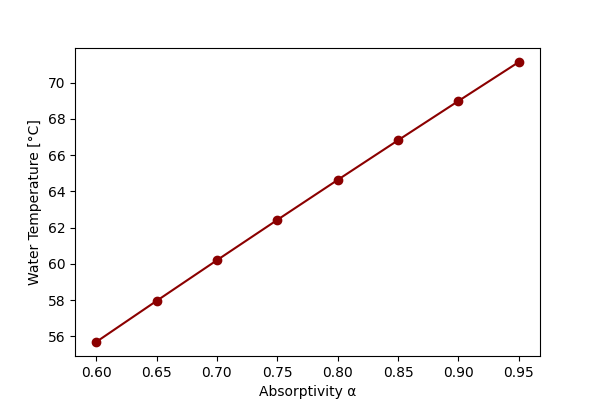
\includegraphics[width=0.7\textwidth]{figures/alpha_2.png}
\caption{Sensitivity of water temperature to changes in absorptivity coefficient ($\alpha$).}
\end{figure}

\begin{figure}[H]
\centering
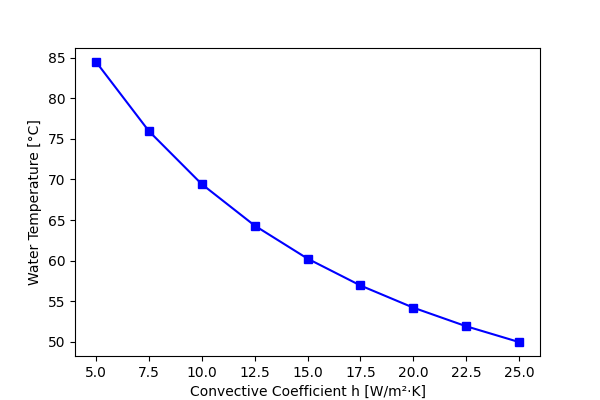
\includegraphics[width=0.7\textwidth]{figures/convection_2.png}
\caption{Sensitivity of water temperature to changes in convection coefficient ($h$).}
\end{figure}

\subsubsection*{Sensitivity Analysis Commentary}
\begin{itemize}
    \item \textbf{Effect of Absorptivity ($\alpha$):} Water temperature increases nearly linearly with absorptivity. Higher $\alpha$ means more solar energy absorbed, leading to higher steady-state temperatures. Changing $\alpha$ from 0.6 to 0.95 can increase $T_w$ by over 20°C, so $\alpha$ is a critical parameter for heating efficiency.
    \item \textbf{Effect of Convection Coefficient ($h$):} Higher $h$ values increase heat loss, lowering water temperature. Sensitivity decreases at high $h$, as convection dominates the heat loss mechanism.
    \item \textbf{Radiative Contribution:} Radiation depends on $T_s^4$, so its relative importance increases with surface temperature. For moderate solar heating, radiation and convection are comparable.
    \item \textbf{Implications:} 
    \begin{itemize}
        \item A breezy environment (higher $h$) can reduce the heating efficiency significantly.
        \item Increasing absorptivity is more effective than reducing convection at low $h$, but less impactful when $h$ is already large.
    \end{itemize}
\end{itemize}

\section*{Appendix: Numerical Solution Code}
This code uses a simple iterative method to solve for the surface temperature $T_s$ based on the energy balance.

\begin{verbatim}
import numpy as np
from scipy.optimize import fsolve
import matplotlib.pyplot as plt

# -------------------------------
# GIVEN PROPERTIES
# -------------------------------
T_inf = 300           # Ambient air temperature [K]
sigma = 5.67e-8       # Stefan-Boltzmann constant [W/m^2/K^4]
alpha_nom = 0.91      # Absorptivity
epsilon = 0.94        # Emissivity
q_solar = 800         # Solar irradiance [W/m^2]
h_nom = 10            # Convective coefficient [W/m^2/K]

# -------------------------------
# ENERGY BALANCE FUNCTION
# -------------------------------
def energy_balance(Ts, alpha, epsilon, q_solar, h, T_inf):
    return alpha*q_solar - h*(Ts - T_inf) - epsilon*sigma*(Ts**4 - T_inf**4)

# -------------------------------
# BASE CASE
# -------------------------------
T_w_base = fsolve(lambda T: energy_balance(T, alpha_nom, epsilon, q_solar, h_nom, T_inf), T_inf)[0]
print("Steady-state water temperature: {:.1f} K ({:.1f} C)".format(T_w_base, T_w_base - 273.15))

# -------------------------------
# SENSITIVITY ANALYSIS 1: Absorptivity
# -------------------------------
alpha_values = np.linspace(0.6, 0.95, 8)
T_w_alpha = [fsolve(lambda T: energy_balance(T, a, epsilon, q_solar, h_nom, T_inf), T_inf)[0] for a in alpha_values]

plt.figure(figsize=(6,4))
plt.plot(alpha_values, np.array(T_w_alpha)-273.15, marker='o', color='darkred')
plt.xlabel("Absorptivity alpha")
plt.ylabel("Water Temperature (C)")
plt.grid(False)
plt.show()

# -------------------------------
# SENSITIVITY ANALYSIS 2: Convection
# -------------------------------
h_values = np.linspace(5, 25, 9)
T_w_h = [fsolve(lambda T: energy_balance(T, alpha_nom, epsilon, q_solar, h_val, T_inf), T_inf)[0] for h_val in h_values]

plt.figure(figsize=(6,4))
plt.plot(h_values, np.array(T_w_h)-273.15, marker='s', color='blue')
plt.xlabel("Convective Coefficient h [W/m^2/K]")
plt.ylabel("Water Temperature (C)")
plt.grid(False)
plt.show()
\end{verbatim}

\end{document}
